\section{机器阅读理解任务概述}

%\footnotetext[1]{\url{www.cnn.com}}\label{1}

机器阅读理解任务是为了使得计算机具有对自然语言文本理解的能力,像人类一样阅读并且理解一篇文章。具体的就是给定
一篇文章$P$和一些与文章$P$相关的问题$Q$,
要求模型通过阅读$P$之后给出$Q$的正确答案$A$,即建模给定$P$和$Q$的条件下预测$A$的概率:
\begin{equation}
    P(A|P,Q)
\end{equation}
根据答案形式的不同,任务也是多种多样的,
大致可以概括为4类:完形填空、多项选择、片段选择和自由回答。
下面对这四种任务分别进行叙述并介绍相关的数据集。


% \begin{table*}[!ht]\tiny
%     \caption{CNN\&Daily Mail数据集中的一个样例}
%     %\centering
%     \vspace{10pt}
%     \resizebox{\textwidth}{!}{
%     \small
%     \begin{tabular}{l}
%         \hline
%         完型填空型数据集 \\
%         \toprule
%         \hspace{-13pt} \textbf{Context} \\
%         The BBC producer allegedly struck by Jeremy \\
% Clarkson will not press charges against the “Top \\
% Gear” host, his lawyer said Friday. Clarkson, who \\
% hosted one of the most-watched television shows \\
% in the world, was dropped by the BBC Wednesday \\
% after an internal investigation by the British broad- \\
% caster found he had subjected producer Oisin Tymon \\
% “to an unprovoked physical and verbal attack.” . . . \\
%         \midrule
%         \hspace{-13pt} \textbf{Query} \\
%         Producer X will not press charges against Jeremy \\
%         Clarkson, his lawyer says.\\
%         \midrule
%         \hspace{-13pt} \textbf{Anwser} \\
%         Oisin Tymon\\
% \bottomrule
        
%     \end{tabular}
%     }

% \end{table*}

% \begin{center}
%     \begin{table}\tiny
%         \caption{完形填空型数据集}
%     \begin{

%     \end{table}
% \end{center}














\subsection{完形填空}
完型填空型阅读理解是指给定一篇文章$P$和一个与文章相关的问题$Q$,$Q$是通过删除
掉句子中某一个单词构成,要求模型根据$P$能够
正确的填写出$Q$缺失的单词。CNN和Daily Mail数据集\upcite{Teaching Machines to Read and Comprehend}是
由Google DeepMind和牛津大学发布于2015年,
这是第一个较大规模的阅读理解型数据集。从CNN\footnote{www.cnn.com\label{cnn}}中收集93k篇文章,从
Daily Mail\footnote{www.dailymail.co.uk\label{daily mail}}上收集220k篇文章。每一篇文章
的作者都为这篇总结出一些具有概括性的句子,这些句子涵盖了这篇文章的要点。于是把这些概括性的句子删去其中的一个单词,
以此作为问题,构建了(文章-问题-答案)的三元组形式的语料库作为填空式的阅读理解任务。

% Children's Book Test(CBT)数据集\upcite{CBT}的构建是Facebook人工智能实验室bAbI
% 项目\footnote{https://research.fb.com/downloads/babi/\label{CBT}}的一部分。在CBT中所用到的书籍
% 来源于项目Project Guntenberg\footnote{https://www.gutenberg.org\label{book}}。对于书中的每篇文章,
% 选取21个连续的句子,前20个句子最为上下文段落,第21个句子挖掉其中的一个单词作为问题,给出10个单词作为候选答案,
% 要求模型从中选取正确的答案。
% CBT数据集与CNN/Daily Mail\upcite{Teaching Machines to Read and Comprehend}数据集构造的方式略有不同,
% CNN/Daily Mail中仅仅只将句子中的某个命名实体单词去掉,其余的命名实体单词用特殊的标记取代然后每次训练都要随机打乱,
% CBT一共去掉四种类型的单词,命名实体、常见的名词、动词、介词,从而形成四种类型的问题,对应着的答案也自然是四种类型。
% 同时对于每种类型的答案,从对应的文章和问题中选取出九个和这个答案一样词性的单词从而构成十个候选答案。

%\end{multicols}
% \begin{center}
%     \textbf{表1: 原始版本vs匿名版本}
%     \begin{tabular}{l l}
%         \toprule
%         Original Version&Anonymised Version \\
%         \midrule
%         \hspace{-13pt} \textbf{\zihao{4} Context} \\
%         The BBC producer allegedly struck by Jeremy&the ent381 producer allegedly struck by ent212 will \\
% Clarkson will not press charges against the “Top&not press charges against the “ ent153 ” host , his \\
% Gear” host, his lawyer said Friday. Clarkson, who&lawyer said friday . ent212 , who hosted one of the \\
% hosted one of the most-watched television shows&most - watched television shows in the world , was\\
% in the world, was dropped by the BBC Wednesday&dropped by the ent381 wednesday after an internal \\
% after an internal investigation by the British broad-&investigation by the ent180 broadcaster found he \\
% caster found he had subjected producer Oisin Tymon&had subjected producer ent193 “ to an unprovoked \\
% “to an unprovoked physical and verbal attack.” . . .&physical and verbal attack . ” . . . \\
%         \midrule
%         \hspace{-13pt} \textbf{\zihao{4} Query} \\
%         Producer X will not press charges against Jeremy&producer X will not press charges against ent212 ,\\
%         Clarkson, his lawyer says.&his lawyer says .\\
%         \midrule
%         \hspace{-13pt} \textbf{\zihao{4} Anwser} \\
%         Oisin Tymon&ent193\\
% \bottomrule
        
%     \end{tabular}
% \end{center}

% \begin{figure}
%     \centering
%     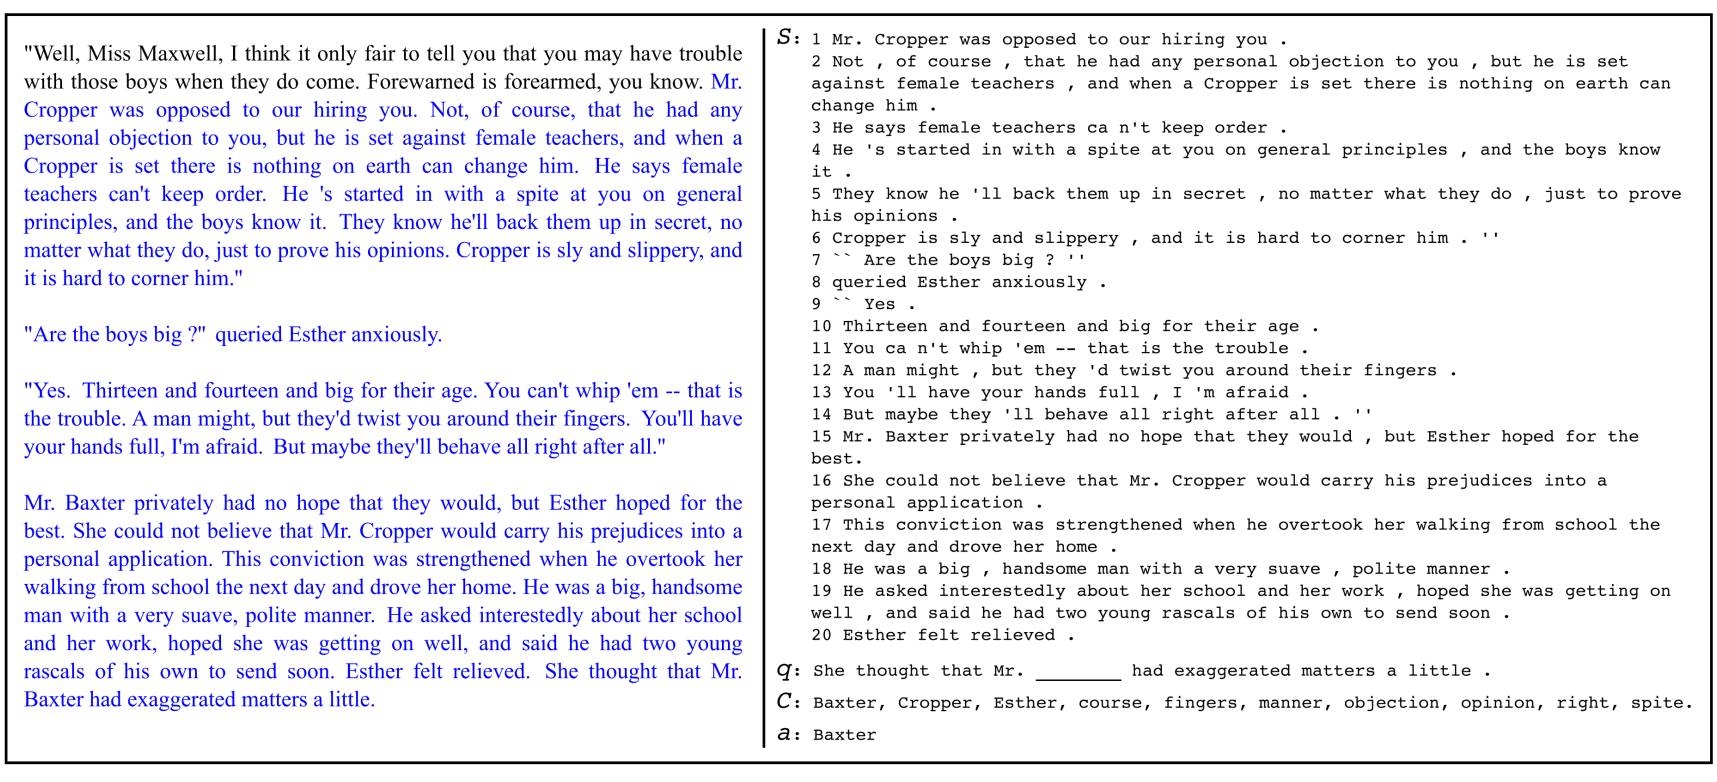
\includegraphics[width=0.2\linewidth]{CBT.png}
%     \caption{CBT数据集样例}
% \end{figure}
% \begin{multicols}{2}
\subsection{多项选择}
多项选择型这类问答任务是对于给定的文$P$,以及和$P$相关的问题$Q$和多个
候选答案$A=\{A_1,A_2,\cdots,A_n\}$,
从中选择正确的答案,即$P(A_i|P,Q)$,其中$A_i \in A$。
相关的数据集如RACE\footnote{www.cs.cmu.edu/glail/data/race/\label{race}},这个数据集是从中
国中学生的英语考试题中
建立的数据集。共有将近28000篇文章以及100000个问题,答案并不是简单的限制于
文章中的单词,而且答案和问题中单词可能
从没有在文中出现过,因此简单的利用单词匹配方式并不能达到很好的效果。
这些问题和候选的答案都是由出题专家生成的,因此更加的
接近真实世界的语义。另外RACE数据集中文章主题的覆盖度比其它的数据集更广泛,比如CNN/Daily\upcite{Teaching Machines to Read and Comprehend}
所有文章全都是来源于CNN新闻,SQuAD\upcite{SQuAD1}数据集所有的文章全都是来源于维基百科。
而RACE数据集涵盖多个领域如新闻、故事、广告、传记等等。由于其类型的多样性因此可以更好的评估机器的阅读理解
能力。

% \begin{wrapfigure}[15]{r}[\dimexpr 1\columnwidth+\columnsep\relax]{0.5\textwidth}%[htbp]
%     \centering
%     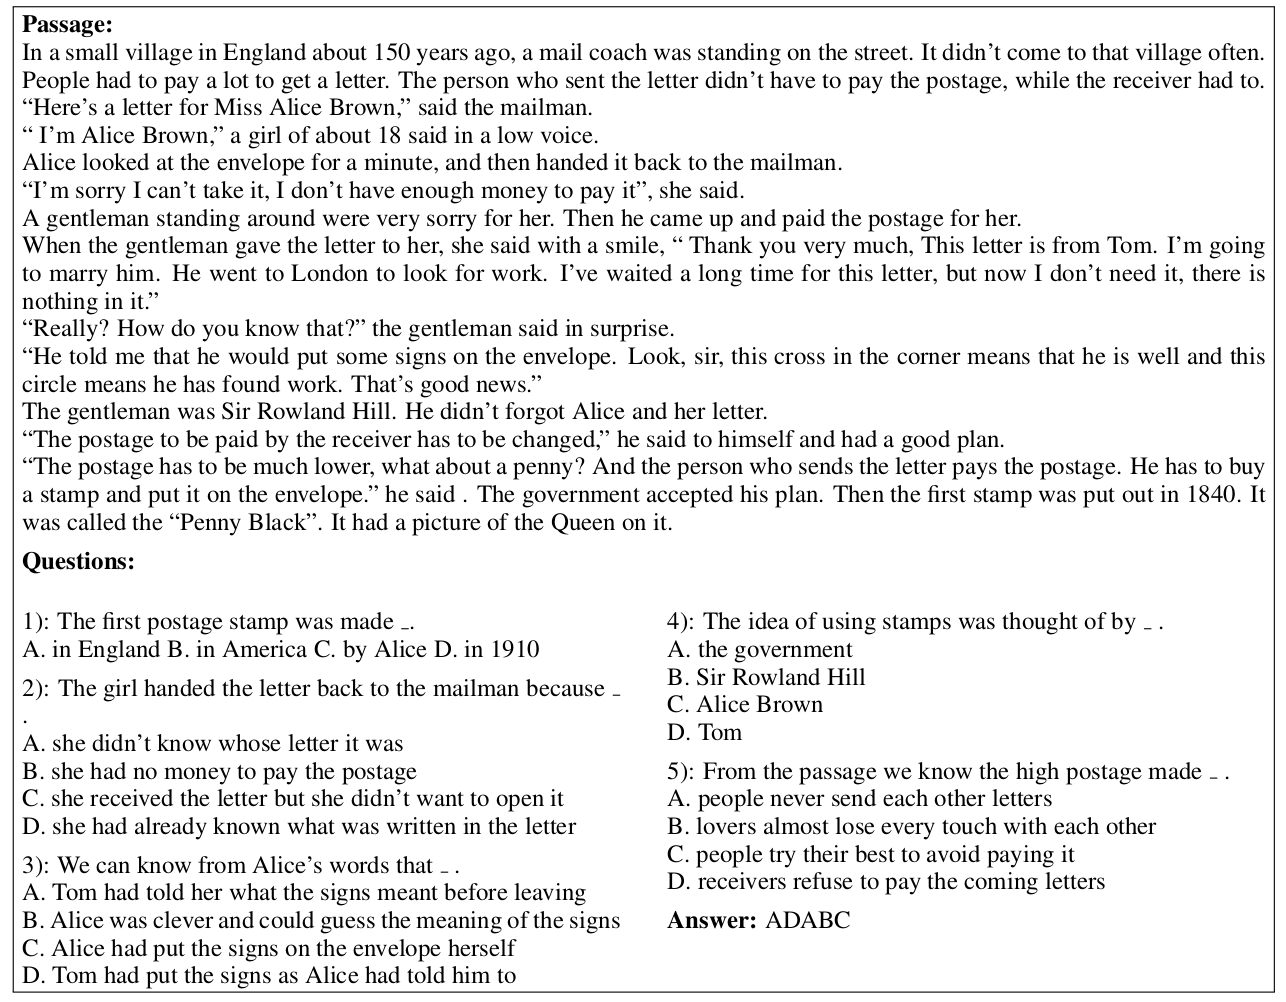
\includegraphics[width=0.5\textwidth]{race.png}
%     \caption{RACE数据集样例\upcite{RACE}}
% \end{wrapfigure}


\subsection{片段选择}
这类问答任务是MRC领域较为流行的研究方向,给出$P$和问题$Q$,问题的答案是$P$中的一段连续的单词构成,
答案的长度不固定,可以表示为$P(A|P,Q)$,其中$A=\{t_i,t_{i+1},\cdots,t_{i+k}\}(1\leq i\leq i+k\leq n)$,$n$代表$P$中
单词的个数。抽取式问答任务最为
广泛使用的数据集是SQuAD 1.1\upcite{SQuAD1}和SQuAD 2.0\upcite{SQuAD2}。其中
SQuAD 1.1是Stanford问答数据集的第一个版本,
由众包工人在维基百科上面的文章中给出问题,答案来源于文章中某段连续的单词。
SQuAD 1.1含有536篇文章,总计107785个问题-答案对。
在SQuAD 2.0中又在原有的数据集中加入了50000多个没有答案的问题,准确的说
这些问题的答案不在相应的文章中。

%\end{multicols}


% \begin{figure}[htbp]
%     \centering
%     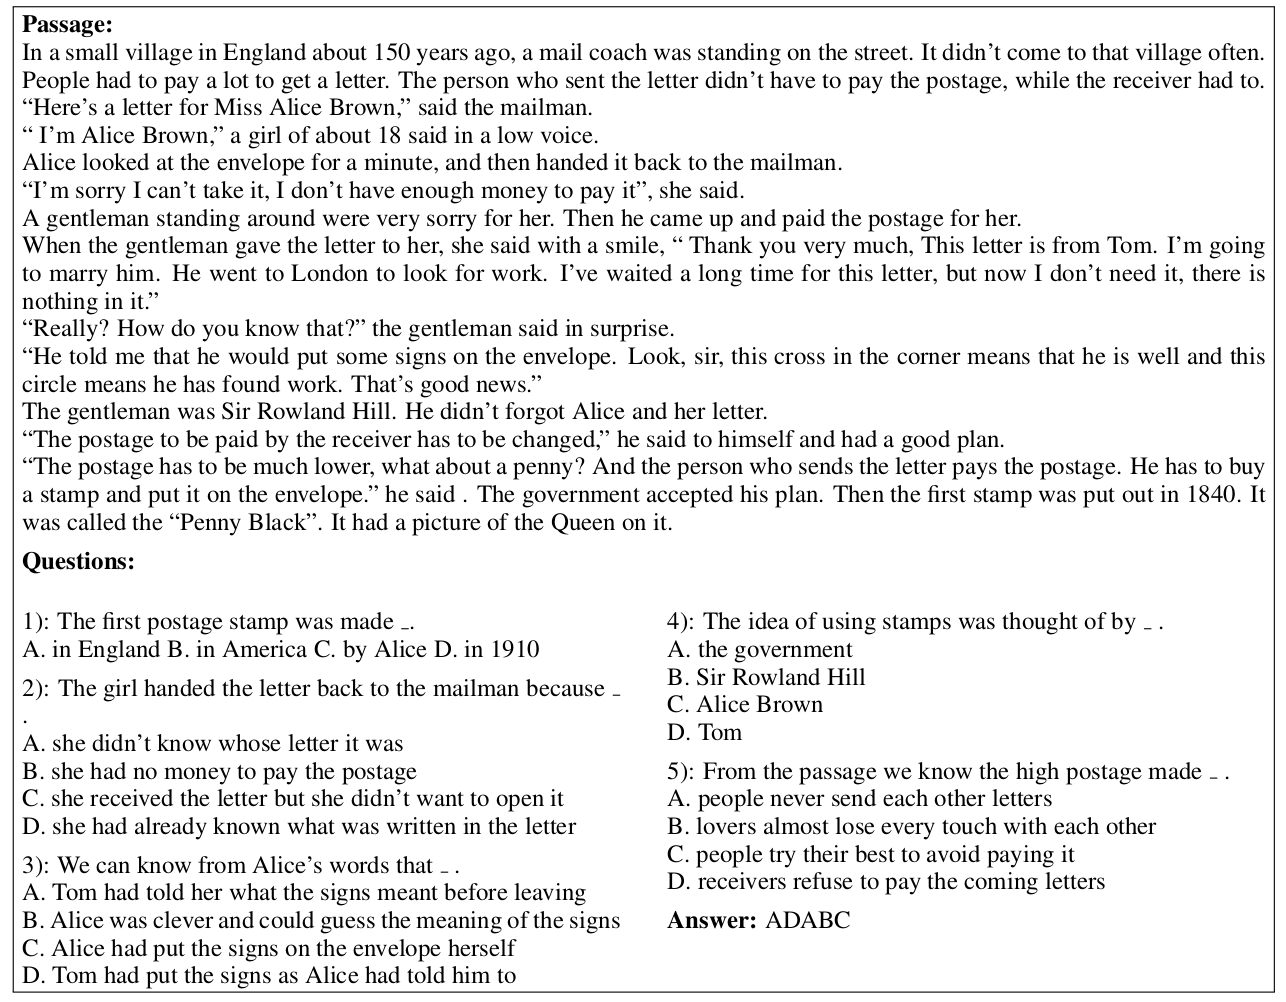
\includegraphics[width=0.5\linewidth]{race.png}
%     \caption{RACE数据集样例\upcite{RACE}}
% \end{figure}

% \begin{figure}
%     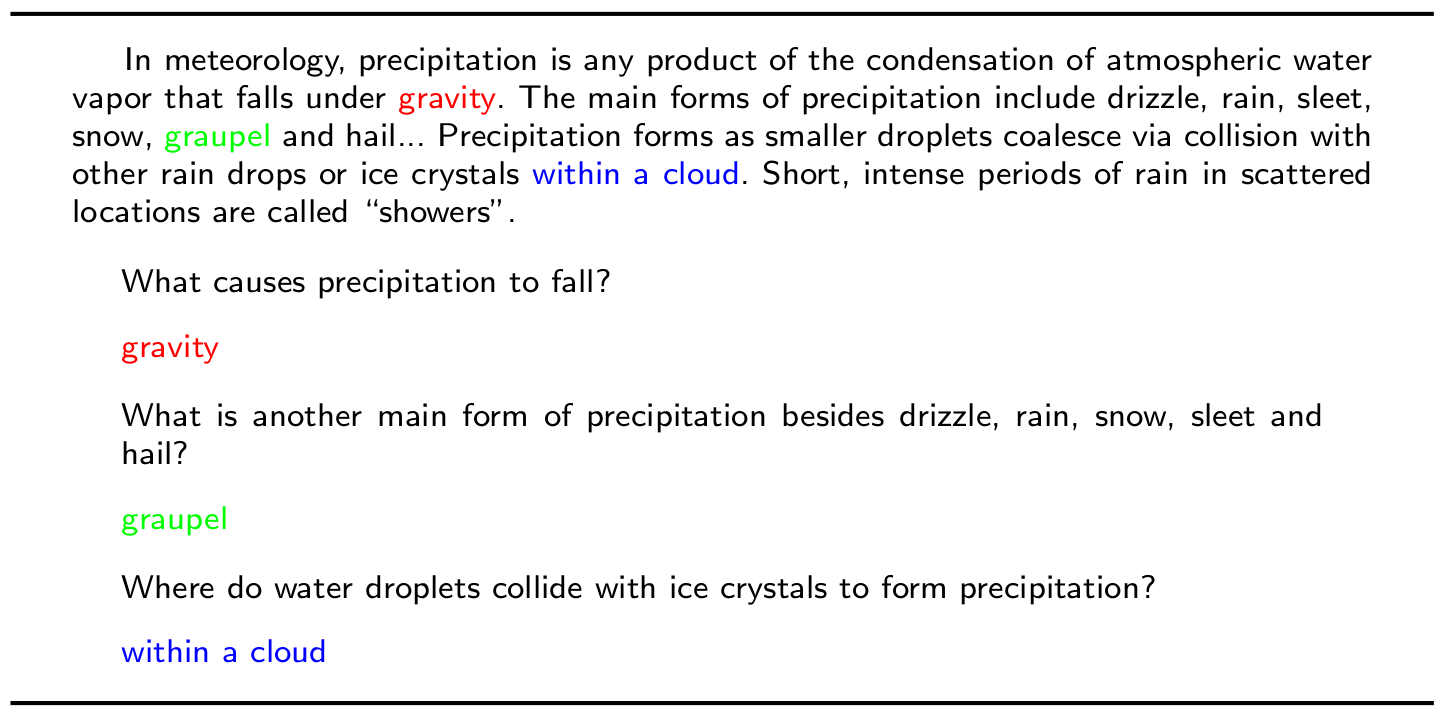
\includegraphics{squadv1.png}
%     \caption{SQuAD v1.0}
% \end{figure}

% \begin{figure}
%     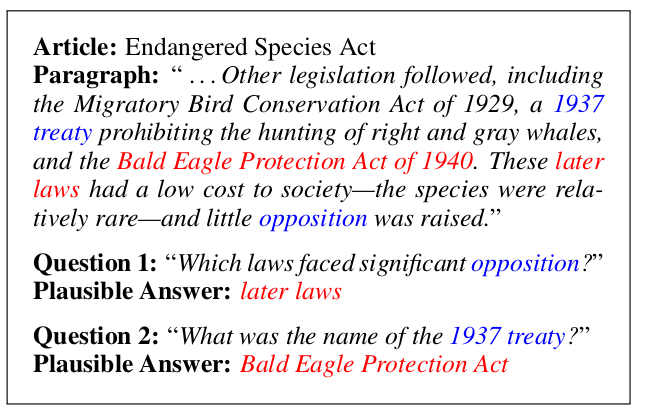
\includegraphics{squad2.png}
%     \caption{SQuAD v2.0}
% \end{figure}


%\begin{multicols}{2}
\subsection{自由回答}
简单的从文章中摘取一段文本可能并不能回答问题需要的答案,自由回答型任务的答案是自由形式的
,不局限于文章中的某些单词,语法上往往是更加的灵活。
可以表示为$P(A|P,Q)$,其中$A\subseteq P$或$A\nsubseteq P$。
从文章中概括提炼出问题的答案也是更加的符合人类的阅读方式的,基于这些原因,自由回答式问答的数据集
也因此公布出来并且受到广泛的关注,
相关的数据集如MS MARCO\upcite{MS marco}。MS MARCO是由微软通过在必应搜素引擎的日志上收集用户
提出的问题,对于文本段落是来源于必应搜素引擎的返回的搜索结果。具体的就是对于每一个问题,给出10个最相关的
查询结果的文本段落,然后由标注人员从这10个文本段落中找出那些与这个问题有关的文本段落,然后人工的从这些选择出来的段落中
概括提炼出答案,同时对于选出来的段落要标记为$is\_select=1$,表示这个段落和答案相关,从而可
以训练模型。

%\vspace{15\baselineskip}
因此可以看到
这个数据集与前面的数据集很大的不同之处就是答案是人工
生成的,不局限于文本段落中固定的一段单词,因此更加的接近现实世界中的人类阅读理解,
对模型的推理能力要求也更高。同时如果不能从给出的10个段落中推理出答案,
那么这个问题就标记为不可回答的问题,同样要保留在数据集中,
目的就是让模型能够判别出问题是否具有答案。
% 如图4为MS MARCO数据集的一个样例。
% %\end{multicols}

% % \begin{wrapfigure}[10]{r}[0em]{0.5\textwidth}%[htbp]
% %     \centering
% %     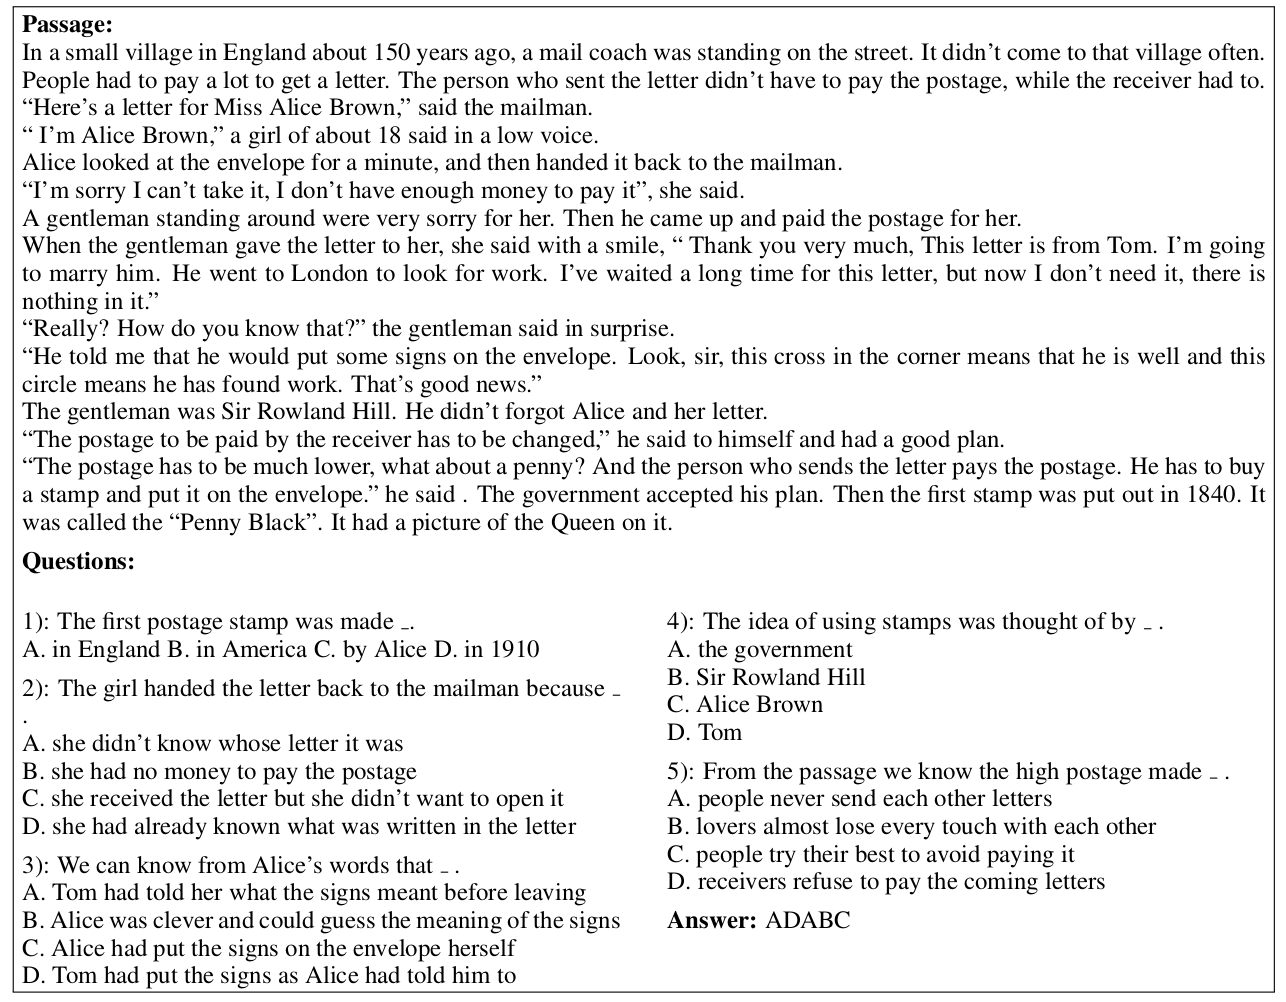
\includegraphics[width=0.5\textwidth]{race.png}
% %     \caption{RACE数据集样例\upcite{RACE}}
% % \end{wrapfigure}

% %\vspace*{5\baselineskip}


% \begin{figure}
%     \centering
%     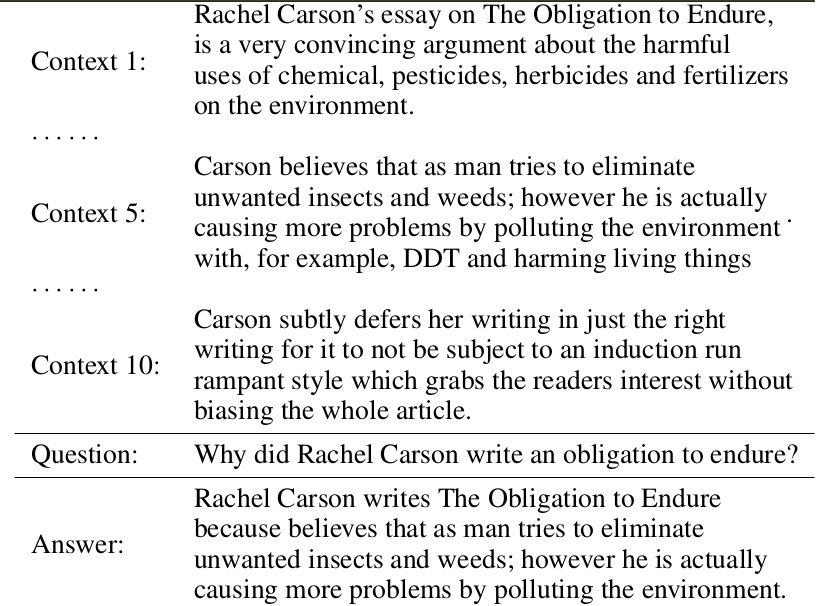
\includegraphics[width=0.8\linewidth]{msmcro.png}
%     \caption{MS marco样例}
% \end{figure}
% \subsection{对话型问答}
% 抽取式问答尽管比填空式问答更复杂,需要模型更强的推理能力,但是这类任务要求答案来源于文章中的一段文本,这样的答案往往不符合现实世界中
% 人与人之间的那种用很短的句子或者单词来回答问题的交互方式。另外简单的从段落中提取出一短文本可能不能回答问题,例如图中的问题4$Q_4$(How many?)。
% 文献\upcite{CoQA}公布了一个用来做对话式问答的数据集,数据集有来源于8千个对话文章的1.26万问题和对应的答案,这些文章取自
% 七种不同的领域包括新闻、考试、维基百科等语料库中收集的文本段落,
% 由提问者给出问题以及回答者给出答案同时给出答案所在的句子或者段落以供模型学习推理,如图所示。可以看出在CoQA数据集中模型必须理解文本段落以及一系列的问题才能给出正确的答案,
% 因为对话中的问题依赖于前面提出的问题和给出的答案,如图中问题5$Q_5$,问题仅仅是Who?所以模型必须理解前面对话中的问题和答案。
% 这种任务的答案是自由式的,不限于任何的文本段落,同样是自由式答案的数据集还有文献\upcite{MS marco},不同的是在CoQA任务中,训练的时候模型要
% 先从文本段落中选出来包含有答案的段落或句子,然后总结概括生成语法形式自由的答案,测试时直接给出答案即可。



% \begin{center}
%     \textbf{Table 1 Anwser type distribution in SQuAD} \\
%     \vspace{5pt}%vspace 是垂直方向拉开距离
%     \begin{tabular}{l l  l}%p{} 设置列宽
%         \toprule
%         Anwser type&Percentage&Example \\
%         \midrule
%         Date&8.9\% &19 Octiber 1512 \\
% Other Numeric&10.9\% &12 \\
% Person&12.9\%&Thomas Coke\\
% Location&4.4\%&Germany\\
% Other Entity&15.3\%&ABC Sports\\
% Common Noun Phrase&31.8\%&property damage\\
% Adjective Phrase&3.9\%&second-largest\\
% Verb Phrase&5.5\%&returned to Earth\\
% Clause&3.7\%&to avoid trivialization\\
% Other&2.7\%&quietly\\
%         \bottomrule
%     \end{tabular}
% \end{center}
% %\vspace{10pt}%vspace 是垂直方向拉开距离
% 从表中可以看出答案的形式是多样的,不仅仅只是单一的名词实体等。至于问题的难度,
% 或者说为了能够得到答案模型所需要的推理能力,作者通过在验证集上的48篇文章中选出来192个问题通过手工的
% 标注出回答每个问题所需要的推理能力,结果表明,每个问题与答案之间都至少存在词汇或语法上的变体,
% 例如同义词变换,多句子推理等。

\subsection{评估方法}
对于不同的MRC任务有不同的评估指标。
对于填空型任务与多项选择型任务都是属于客观题型,用准确率就可以衡量模型的性能。
片段选择型任务属于半客观题型,通常用精确匹配EM(Exact Match)和F1值来评估模型,F1值是精确率和召回率
之间的调和平均数。对于自由回答式任务的答案,一般采用单词水平的匹配率作为评分标准,常用标准有
ROUGE\upcite{ROUGE}。下面详细介绍这几种评估指标如何评估不同的MRC任务。
\subsubsection{准确率}
准确率可以用来评估完形填空和多项选择这两种类型的任务。
对于测试集合中的所有问题$Q=\{Q_1,Q_2,\cdots,Q_m\}$,其中$m$代表问题的个数。如果模型预测出来的
$m$个答案中有$n$个是正确的,那么模型的准确率自然是$n/m$。
精确匹配EM评估指标可以看做是准确率的扩展,就片段选择型任务来讲,EM要求
预测出来的所有单词要和标准答案
的所有单词要精确匹配下,EM值才为1,否则为0。
因此最后模型在测试集上的EM值也就是$n/m$。
\subsubsection{F1}
F1分数是最为普遍使用的一种评估标准,不仅仅局限于MRC的各种任务。
F1值是精确率(precision)和召回率(recall)
之间的调和平均数。
具体计算公式如下:
\begin{equation}
    \text{F1}=\displaystyle\frac{2\times\text{precision}\times\text{recall}}{\text{precision}+\text{recall}}
\end{equation}
精确率是指模型预测的答案中有多大比例的单词是标准答案中的单词。
召回率是指标准答案中的单词有多大比例在预测答案中出现。

\subsubsection{ROUGE}
ROUGE(Recall-Oriented Understudy for Gisting Evaluation)最初是用来
评估生成文本摘要的一种方法,因为可以ROUGE的计算机制
来评估MRC领域中自由答案型任务。ROUGE的评分有多种,在MRC领域较为常用的是ROUGE-L,
ROUGE-L用来计算标准答案和预测答案的最长公共子序列(Longest Common Subsequence,LCS),ROUGE-L的计算
公式如下:
\begin{gather}
    R_{LCS}=\displaystyle\frac{LCS(X,Y)}{m} \\
    P_{LCS}=\displaystyle\frac{LCS(X,Y)}{n} \\
    F_{LCS}=\displaystyle\frac{{(1+\beta)}^2R_{LCS}P_{LCS}}{R_{LCS}+\beta^2P_{LCS}}
\end{gather}
其中$LCS(X,Y)$表示标准答案与预测答案之间的最长公共子序列,
$m$和$n$分别代表标准答案和预测答案中单词的个数,$\beta$是ROUGE-L的的参数,
用来控制精确率和召回率的重要程度。








